\begin{figure}
  \centering
  \hspace*{-0.15\textwidth}%
  \begin{subfigure}[t]{0.125\textwidth}
    \tikzstyle{legend-point}=[circle, inner sep=2pt]
    \definecolor{m-octree}{HTML}{966687}
    \definecolor{r-octree}{HTML}{837150}
    \definecolor{m-data}{HTML}{697b9c}
    \definecolor{r-data}{HTML}{568665}
    
    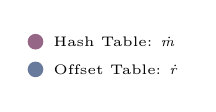
\begin{tikzpicture}
      \node (legend:1) at (0.1\textwidth,   0pt) [legend-point, fill={m-octree}, label=right:{\tiny Hash Table: $\mathit{\dot{m}}$}] {};
      \node (legend:2) at (0.1\textwidth, -10pt) [legend-point, fill={m-data}, label=right:{\tiny Offset Table: $\mathit{\dot{r}}$}] {};
    \end{tikzpicture}
  \end{subfigure}%
  \begin{adjustbox}{minipage=0.4\textwidth, scale=0.6}
    \begin{subfigure}[b]{1.6\textwidth}
      \centering
      \def\svgwidth{\textwidth}
      \input{./img/raw/hs-layered-mem/layered_spaceship-indoor_1260_octree.pdf_tex}
      \caption{Spaceship Indoor}
      \vspace{4pt}
      \label{fig:hs-layered-mem:indoor-octree}
    \end{subfigure}
  \end{adjustbox}\hspace{0.125\textwidth} %
  \begin{adjustbox}{minipage=0.4\textwidth, scale=0.6}
    \begin{subfigure}[b]{1.6\textwidth}
      \centering
      \def\svgwidth{\textwidth}
      \input{./img/raw/hs-layered-mem/layered_pipers-alley_1044_octree.pdf_tex}
      \caption{Piper's Alley}
      \label{fig:hs-layered-mem:alley-octree}
    \end{subfigure}
  \end{adjustbox}
  \caption{\small Number of pixels used by the octree description spatial hash functions per layer of the linkless octree.}
  \label{fig:hs-layered-mem:octree}
  % --------------------------------------------------------------------------------------------------------------------------
  \hspace*{-0.15\textwidth}%
  \begin{subfigure}[t]{0.125\textwidth}
    \tikzstyle{legend-point}=[circle, inner sep=2pt]
    \definecolor{m-octree}{HTML}{966687}
    \definecolor{r-octree}{HTML}{837150}
    \definecolor{m-data}{HTML}{697b9c}
    \definecolor{r-data}{HTML}{568665}
    
    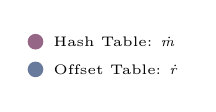
\begin{tikzpicture}
      \node (legend:1) at (0.1\textwidth,   0pt) [legend-point, fill={m-octree}, label=right:{\tiny Hash Table: $\mathit{\dot{m}}$}] {};
      \node (legend:2) at (0.1\textwidth, -10pt) [legend-point, fill={m-data}, label=right:{\tiny Offset Table: $\mathit{\dot{r}}$}] {};
    \end{tikzpicture}
  \end{subfigure}%
  \begin{adjustbox}{minipage=0.4\textwidth, scale=0.6}
    \begin{subfigure}[b]{1.6\textwidth}
      \centering
      \def\svgwidth{\textwidth}
      \input{./img/raw/hs-layered-mem/layered_spaceship-indoor_1260_data.pdf_tex}
      \caption{Spaceship Indoor}
      \vspace{4pt}
      \label{fig:hs-layered-mem:indoor-data}
    \end{subfigure}
  \end{adjustbox}\hspace{0.125\textwidth} %
  \begin{adjustbox}{minipage=0.4\textwidth, scale=0.6}
    \begin{subfigure}[b]{1.6\textwidth}
      \centering
      \def\svgwidth{\textwidth}
      \input{./img/raw/hs-layered-mem/layered_pipers-alley_1044_data.pdf_tex}
      \caption{Piper's Alley}
      \label{fig:hs-layered-mem:alley-data}
    \end{subfigure}
  \end{adjustbox}
  \caption{\small Number of pixels used of the data description spatial hash functions per layer of the linkless octree.}
  \label{fig:hs-layered-mem:data}
  % --------------------------------------------------------------------------------------------------------------------------
  \hspace*{-0.15\textwidth}%
  \begin{subfigure}[t]{0.125\textwidth}
    \tikzstyle{legend-point}=[circle, inner sep=2pt]
    \definecolor{legend1}{HTML}{4c72b0}
    \definecolor{legend2}{HTML}{55a868}
    \definecolor{legend3}{HTML}{c44e52}
    \definecolor{legend4}{HTML}{8172b2}
    \definecolor{legend5}{HTML}{ccb974}
    
    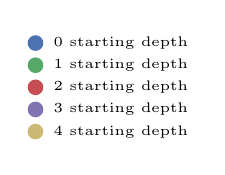
\begin{tikzpicture}
      \node (legend1) at (0.0\textwidth, 0)
            [legend-point, fill={legend1}, label=right:{\tiny $0$ starting depth}] {};
      \node (legend2) at (0.0\textwidth, -8pt)
            [legend-point, fill={legend2}, label=right:{\tiny $1$ starting depth}] {};
      \node (legend3) at (0.0\textwidth, -16pt)
            [legend-point, fill={legend3}, label=right:{\tiny $2$ starting depth}] {};
      \node (legend6) at (0.0\textwidth, -24pt)
            [legend-point, fill={legend4}, label=right:{\tiny $3$ starting depth}] {};
      \node (legend7) at (0.0\textwidth, -32pt)
            [legend-point, fill={legend5}, label=right:{\tiny $4$ starting depth}] {};
    \end{tikzpicture}
  \end{subfigure} %
  \begin{adjustbox}{minipage=0.4\textwidth, scale=0.6}
    \begin{subfigure}[b]{1.6\textwidth}
      \centering
      \def\svgwidth{\textwidth}
      \input{./img/raw/hs-sd-construction-time/construction_sd_time_pipers-alley.pdf_tex}
      \caption{Piper's Alley}
      \vspace{4pt}
      \label{fig:hs-sd-construction:alley}
    \end{subfigure}
  \end{adjustbox} \hspace{0.125\textwidth} %
  %
  \begin{adjustbox}{minipage=0.4\textwidth, scale=0.6}
    \begin{subfigure}[b]{1.6\textwidth}
      \centering
      \def\svgwidth{\textwidth}
      \input{./img/raw/hs-sd-construction-time/construction_sd_time_ziggurat-city.pdf_tex}
      \caption{Ziggurat City}
      \label{fig:hs-sd-construction:city}
    \end{subfigure}
  \end{adjustbox}
  \caption{\small Construction time as function of the starting depth.}
  \label{fig:hs-sd-construction}

  % --------------------------------------------------------------------------------------------------------------------------
  \hspace*{-0.15\textwidth}%
  \begin{subfigure}[t]{0.125\textwidth}
    \tikzstyle{legend-point}=[circle, inner sep=2pt]
    \definecolor{legend1}{HTML}{4c72b0}
    \definecolor{legend2}{HTML}{55a868}
    \definecolor{legend3}{HTML}{c44e52}
    \definecolor{legend4}{HTML}{8172b2}
    \definecolor{legend5}{HTML}{ccb974}
    
    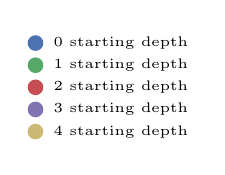
\begin{tikzpicture}
      \node (legend1) at (0.0\textwidth, 0)
            [legend-point, fill={legend1}, label=right:{\tiny $0$ starting depth}] {};
      \node (legend2) at (0.0\textwidth, -8pt)
            [legend-point, fill={legend2}, label=right:{\tiny $1$ starting depth}] {};
      \node (legend3) at (0.0\textwidth, -16pt)
            [legend-point, fill={legend3}, label=right:{\tiny $2$ starting depth}] {};
      \node (legend6) at (0.0\textwidth, -24pt)
            [legend-point, fill={legend4}, label=right:{\tiny $3$ starting depth}] {};
      \node (legend7) at (0.0\textwidth, -32pt)
            [legend-point, fill={legend5}, label=right:{\tiny $4$ starting depth}] {};
    \end{tikzpicture}
  \end{subfigure} %
  \begin{adjustbox}{minipage=0.4\textwidth, scale=0.6}
    \begin{subfigure}[b]{1.6\textwidth}
      \centering
      \def\svgwidth{\textwidth}
      \input{./img/raw/hs-sd-memory/memory_sd_pipers-alley.pdf_tex}
      \caption{Piper's Alley}
      \vspace{4pt}
      \label{fig:hs-sd-memory:alley}
    \end{subfigure}
  \end{adjustbox} \hspace{0.125\textwidth} %
  %
  \begin{adjustbox}{minipage=0.4\textwidth, scale=0.6}
    \begin{subfigure}[b]{1.6\textwidth}
      \centering
      \def\svgwidth{\textwidth}
      \input{./img/raw/hs-sd-memory/memory_sd_ziggurat-city.pdf_tex}
      \caption{Ziggurat City}
      \label{fig:hs-sd-memory:city}
    \end{subfigure}
  \end{adjustbox}
  \caption{\small Number of pixels of the linkless octree as function of the starting depth.}
  \label{fig:hs-sd-memory}
\end{figure}

